\section{Finite subgroups as jet tests}\label{sec:lattice}

We now find an injective jet test for the triangle spaces
$\mathcal M(kP_t)$.  The test points will form a finite subgroup of the
complex torus.  Averaging over this group separates a Laurent polynomial
into components supported on cosets of a sublattice.  In the coordinates
of that sublattice, each component lies in a triangle for which a
one-point multiplicity estimate applies.

\subsection{A multiplicity estimate for triangles}

Gundlach's discussion of varying triangles
\cite[Section~6, Remark~28, Question~29, and Remark~30]{Gundlach2021}
motivated the search for continuously varying triangle interpolation
tests.  The multiplicity estimate used here is proved directly by slices
and Laurent-polynomial factorization, not by a topological argument.

For a bounded subset of $\R^2$, its \emph{vertical range} is the length of
its projection onto the second coordinate axis.  The following estimate
allows arbitrary real vertices and translations.

\begin{lemma}\label{lem:triangle-multiplicity}
Let $\rho>0$, and let $\Delta\subset\R^2$ be a triangle of area
$\rho^2/2$ and vertical range $\rho$.  Every nonzero Laurent polynomial
$F\in\C[U^{\pm1},Z^{\pm1}]$ whose exponent support is contained in
$\Delta$ satisfies
\[
 \ord_{(1,1)}F\leq\rho.
\]
\end{lemma}

\begin{figure}[htbp]
\centering
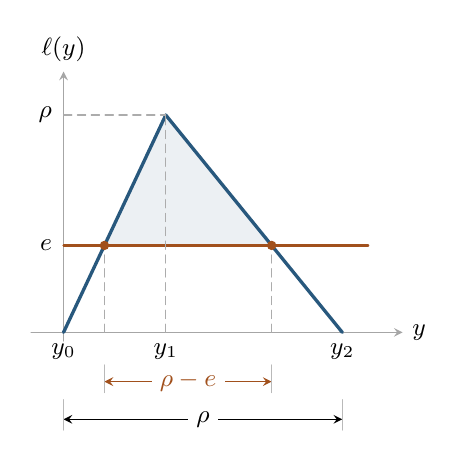
\begin{tikzpicture}[x=1.18cm,y=.92cm,font=\small,
  line cap=round,line join=round,>=stealth]
  \definecolor{sliceblue}{RGB}{40,88,125}
  \definecolor{sliceorange}{RGB}{161,80,28}
  \fill[sliceblue!9] (.44,1.2)--(1.1,3)--(2.24,1.2)--cycle;
  \draw[->,gray!70] (-.35,0)--(3.65,0) node[right,text=black] {$y$};
  \draw[->,gray!70] (0,-.12)--(0,3.6) node[above,text=black] {$\ell(y)$};
  \draw[sliceblue,very thick] (0,0)--(1.1,3)--(3,0);
  \draw[densely dashed,gray!65] (0,3)--(1.1,3);
  \draw[sliceorange,thick] (0,1.2)--(3.28,1.2);
  \draw[densely dashed,gray!65] (.44,0)--(.44,1.2)
    (2.24,0)--(2.24,1.2) (1.1,0)--(1.1,3);
  \fill[sliceorange] (.44,1.2) circle (1.7pt) (2.24,1.2) circle (1.7pt);
  \node[left,inner sep=4pt] at (0,3) {$\rho$};
  \node[left,inner sep=4pt] at (0,1.2) {$e$};
  \node[below,inner sep=4pt] at (0,0) {$y_0$};
  \node[below,inner sep=4pt] at (1.1,0) {$y_1$};
  \node[below,inner sep=4pt] at (3,0) {$y_2$};
  \draw[<->,sliceorange] (.44,-.68)--(2.24,-.68)
    node[midway,fill=white,inner sep=3pt] {$\rho-e$};
  \draw[gray!55] (.44,-.45)--(.44,-.83) (2.24,-.45)--(2.24,-.83);
  \draw[<->] (0,-1.20)--(3,-1.20)
    node[midway,fill=white,inner sep=3pt] {$\rho$};
  \draw[gray!55] (0,-.93)--(0,-1.35) (3,-.93)--(3,-1.35);
\end{tikzpicture}
\caption{Horizontal slice lengths of a triangle of area $\rho^2/2$
and vertical range $\rho$. The tent has height $\rho$. For
$0\le e\le\rho$, the heights in the vertical projection at which
$\ell(y)\ge e$ form an interval of length $\rho-e$.
The graph shows three distinct vertex heights; a horizontal side gives
the same conclusion with a one-sided tent.}
\label{fig:triangle-slices}
\end{figure}


\begin{proof}
For a height $y$ in the vertical projection of $\Delta$, let $\ell(y)$
be the horizontal length of the slice of $\Delta$ at that height.  Write
$y_0\leq y_1\leq y_2$ for the three vertex heights; thus
$y_2-y_0=\rho$.  If these heights are distinct, $\ell$ increases linearly
from zero at $y_0$ to its maximum at $y_1$, then decreases linearly to
zero at $y_2$.  If two vertex heights coincide, $\Delta$ has a horizontal
side and there is just one linear segment.  In either case, the area is
one half the vertical range times the maximum slice length.  The maximum
is therefore $\rho$.

More precisely, for $0\leq e\leq\rho$, the heights with
$\ell(y)\geq e$ form an interval of length $\rho-e$
(Figure~\ref{fig:triangle-slices}).  When the three
heights are distinct, its endpoints are
\[
 y_0+\frac e\rho(y_1-y_0),
 \qquad
 y_2-\frac e\rho(y_2-y_1).
\]
The same formulas apply when two adjacent heights coincide, including
the cases $e=0$ and $e=\rho$.

Write $F=\sum_q f_q(U)Z^q$, with each displayed row $f_q$ nonzero, and
let $e$ be the least order of these rows at $U=1$.  Dividing every row by
$(U-1)^e$ gives
\[
 F=(U-1)^eD,
 \qquad D=\sum_q d_q(U)Z^q,
 \qquad D(1,Z)\ne0.
\]
Indeed, at least one $d_q(1)$ is nonzero, and distinct powers of $Z$ are
linearly independent.  All $d_q$ remain Laurent polynomials, including
when some exponents are negative.

The horizontal exponent span of the row
$f_q=(U-1)^e d_q$ is exactly $e$ plus that of $d_q$: the extreme
coefficients of the product are nonzero.  Thus $\ell(q)\geq e$ for every
height occurring in $D$.  There is no cancellation between distinct
heights, since the multiplying factor depends only on $U$.  It follows
that $e\leq\rho$ and that the heights occurring in $D$ span an interval
of length at most $\rho-e$.

On setting $U=1$, some rows may disappear, but no new height appears.
The nonzero Laurent polynomial $D(1,Z)$ therefore has exponent span at
most $\rho-e$.  Multiplication by a power of $Z$, which is a unit at
$Z=1$, turns it into an ordinary polynomial of degree at most
$\rho-e$.  Consequently
\[
 \ord_{(1,1)}D
 \leq \ord_1 D(1,Z)
 \leq \rho-e.
\]
The first inequality holds because restriction cannot introduce a term
of smaller total degree into the local Taylor series.  Orders add under
products of nonzero holomorphic germs, so $\ord_{(1,1)}F\leq\rho$.
All exponent spans and orders used here are integers; no integrality of
$\rho$, the vertices, or the translating vector is required.
\end{proof}


\subsection{The subgroup test}

For integer vectors $u,\xi\in\Z^2$, write $\det(u,\xi)$ for their
oriented determinant, extending this notation linearly to real $\xi$.
A vector in $\Z^2$ is \emph{primitive} if its coordinates are coprime.

\begin{proposition}\label{prop:subgroup-test}
Let $H>0$, let $r$ be a positive integer, and let $P\subset\R^2$ be a
triangle of area $H/2$.  Suppose there is a primitive vector $u\in\Z^2$
such that
\[
 \max_{\xi\in P}\det(u,\xi)
 -\min_{\xi\in P}\det(u,\xi)=\sqrt{rH}.
\]
Then there is a subgroup $G\subset\T$ of exactly $r$ distinct points
such that, for all positive integers $k,m$ with
$m>k\sqrt{H/r}$, the order-$m$ jet test on $\mathcal M(kP)$ at $G$ is
injective.
\end{proposition}

\begin{proof}
Complete $u$ to an integer basis $(u,v_0)$ with $\det(u,v_0)=1$.
Put $v=rv_0$ and
\[
 M=\Z u+\Z v\subset\Z^2.
\]
This sublattice has index $r$.  For $\eta=(\eta_1,\eta_2)\in\Z^2$,
write $\chi_\eta(x,z)=x^{\eta_1}z^{\eta_2}$ for the corresponding
character on $\T$, and define
\[
 G=\{p\in\T:\chi_\eta(p)=1\text{ for every }\eta\in M\}.
\]
The characters $X=\chi_u$ and $Y=\chi_{v_0}$ are torus coordinates:
their exponent matrix is unimodular, so its inverse also has integer
entries.  In these coordinates,
\[
 G=\{(X,Y):X=1,\ Y^r=1\}.
\]
Over $\C$, this consists of exactly $r$ distinct points.

Suppose, toward a contradiction, that a nonzero
$f\in\mathcal M(kP)$ has order at least $m$ at every point of $G$.
For $g\in G$, let $(\tau_gf)(p)=f(gp)$.  Translation by $g$ permutes
$G$ and is locally invertible, so every $\tau_gf$ has the same prescribed
vanishing.  For a coset $\eta+M$, its character projection is
\[
 f_\eta=\frac1r\sum_{g\in G}\chi_\eta(g)^{-1}\tau_gf.
\]
This is exactly the sum of the monomials of $f$ with exponents in
$\eta+M$.  Indeed, if $\xi-\eta=n u+\ell v_0$, then
$\chi_{\xi-\eta}$ restricts to $\zeta^\ell$ on $G$.  The sum over the
$r$th roots of unity gives
\[
 \frac1r\sum_{g\in G}\chi_{\xi-\eta}(g)
 =\begin{cases}
 1,&\xi-\eta\in M,\\
 0,&\xi-\eta\notin M.
 \end{cases}
\]
Thus the displayed projection keeps precisely the required coset.
Each $f_\eta$ still has order at least $m$ at every point of $G$, and its
support remains inside $kP$.  Since the components sum to $f$, choose
one that is nonzero.

Multiplication by the Laurent monomial $\chi_{-\eta}$ preserves local
orders and shifts this component's support into $M$.  There is therefore
a nonzero Laurent polynomial $F$ such that
\[
 \chi_{-\eta}f_\eta=F(U,Z),
 \qquad U=\chi_u,
 \qquad Z=\chi_v=Y^r.
\]
The map $(x,z)\mapsto(U,Z)$ is locally invertible at the identity:
in coordinates $(X,Y)$ it is $(X,Y)\mapsto(X,Y^r)$, whose derivative at
$(1,1)$ is $\operatorname{diag}(1,r)$.  The complex inverse function theorem therefore makes it a biholomorphism
on sufficiently small analytic neighborhoods.  In particular,
\[
 \ord_{(1,1)}F
 =\ord_{(1,1)}(\chi_{-\eta}f_\eta)\geq m.
\]
Only local invertibility is used; the map need not be injective on the
whole torus.

Let $N$ be the matrix with columns $u,v$.  The exponent support of $F$
lies in the real triangle
\[
 \Delta=N^{-1}(kP-\eta).
\]
Since $\det N=r$, this triangle has area $k^2H/(2r)$.  The second
coordinate of $N^{-1}\xi$ is $\det(u,\xi)/r$, so its vertical range is
$k\sqrt{rH}/r=k\sqrt{H/r}$.  Translation by $\eta$ changes neither
calculation.  Lemma~\ref{lem:triangle-multiplicity}, with
$\rho=k\sqrt{H/r}$, now gives
$\ord_{(1,1)}F\leq k\sqrt{H/r}<m$, the required contradiction.
\end{proof}

\subsection{A direction for every sufficiently large integer}

We apply Proposition~\ref{prop:subgroup-test} to
\[
 P_t=\conv\{(-b,0),(a,0),(0,1/d)\},
 \qquad
 a=\frac{dHt}{1+t},\quad b=\frac{dH}{1+t},\quad t>T,
\]
with $d,H,T$ fixed in Section~\ref{sec:node}.  Every triangle in this
family has area $H/2$, since $a+b=dH$.  Varying $t$ continuously will
make its determinant projection have the exact length needed for each
large $r$.

\begin{lemma}\label{lem:direction}
Fix $d,H>0$ and $T>1$, and define $P_t$ as above for $t>T$.
For every sufficiently large integer $r$ there are $t>T$ and a primitive
vector $u\in\Z^2$ such that the range of $\det(u,\cdot)$ on $P_t$ has
length $\sqrt{rH}$.  The threshold depends only on $d,H,T$.
\end{lemma}

\begin{proof}
Put $W=dH$ and $a_0=WT/(1+T)$.  As $t$ ranges over $(T,\infty)$,
$a=Wt/(1+t)$ ranges continuously and bijectively over $(a_0,W)$.
For $R=\sqrt{rH}$ sufficiently large, choose $j$ to be the largest power
of two at most $R/(2W)$.  Then
\[
 \frac{R}{4W}<j\leq\frac{R}{2W},
 \qquad jW<R.
\]
The open interval
\[
 I_r=\bigl(d(R-jW),\ d(R-ja_0)\bigr)
\]
has length
\[
 dj(W-a_0)>\frac{dR}{4(1+T)},
\]
which exceeds $2$ for every sufficiently large $r$.  Hence $I_r$
contains an odd integer $i$.  Its lower endpoint is positive, so $i>0$;
as $j$ is a power of two, the vector $u=(i,j)$ is primitive.

The strict inequalities defining $I_r$ imply
\[
 a_*:=\frac{R-i/d}{j}\in(a_0,W).
\]
Choose the unique $t>T$ for which $a=a_*$.  Since $b=W-a$, we have
\[
 \frac{i}{d}+ja=R,
 \qquad
 \frac{i}{d}-jb=R-jW>0.
\]
The determinant functional has the three vertex values
\[
 \det\bigl(u,(-b,0)\bigr)=jb,
 \qquad
 \det\bigl(u,(a,0)\bigr)=-ja,
 \qquad
 \det\bigl(u,(0,1/d)\bigr)=\frac{i}{d}.
\]
Its minimum is therefore $-ja$ and its maximum is $i/d$, giving the
required range $R$ exactly.  All lower bounds on $r$ in this construction
depend only on the fixed data $d,H,T$.
\end{proof}

\begin{corollary}\label{cor:torus-test}
For the fixed parameters $d,H,T$ of Section~\ref{sec:node}, there is an
integer $r_0$ such that for every integer $r\geq r_0$ one can choose a
single $t>T$ and a subgroup $G\subset\T$ of $r$ distinct points for
which the following holds: for all positive integers $k,m$ satisfying
\[
 m>k\sqrt{H/r},
\]
the order-$m$ jet test on $\mathcal M(kP_t)$ at $G$ is injective.
\end{corollary}

\begin{proof}
First fix $r$ and choose $t$ and $u$ by Lemma~\ref{lem:direction}.
The area of $P_t$ is $H/2$, so Proposition~\ref{prop:subgroup-test}
produces $G$ with the stated property simultaneously for all $k,m$.
Thus $r_0$, and then $t,G$, are chosen before these two jet parameters.
\end{proof}

Corollary~\ref{cor:surface-transfer} now gives a surface configuration
with the same injective jet test for each pair $k,m$.  These configurations
may depend on the pair.  The next section passes to very general points
where all the tests hold at once, and uses them to prove nefness.
